\documentclass[aspectratio=1610,10pt]{beamer}
\usetheme{default}
\usecolortheme{default}
\setbeamertemplate{navigation symbols}{}
\setbeamertemplate{footline}[frame number]

\usepackage[utf8]{inputenc}
\usepackage[T1]{fontenc}
\usepackage[provide=*,ngerman]{babel}
\usepackage{lmodern}
\usepackage{graphicx}
\usepackage{booktabs}
\usepackage{array}
\usepackage{tikz}
\usetikzlibrary{positioning,arrows.meta,calc,fit}
\usepackage{amsmath}

\definecolor{navy}{HTML}{17223B}
\definecolor{blueaccent}{HTML}{2E5E9E}
\definecolor{greenaccent}{HTML}{2B7A57}
\definecolor{lightbg}{HTML}{F6F8FC}
\definecolor{linegray}{HTML}{AEB7C3}
\definecolor{softgreen}{HTML}{E8F3EE}
\definecolor{softblue}{HTML}{EAF1FA}

\setbeamercolor{background canvas}{bg=lightbg}
\setbeamercolor{frametitle}{fg=navy}
\setbeamercolor{title}{fg=navy}
\setbeamercolor{structure}{fg=blueaccent}
\setbeamerfont{frametitle}{series=\bfseries,size=\Large}
\setbeamerfont{title}{series=\bfseries,size=\Large}
\setbeamerfont{normal text}{size=\small}
\setbeamertemplate{itemize item}{\color{blueaccent}$\blacktriangleright$}
\setbeamertemplate{enumerate item}{\color{blueaccent}\insertenumlabel.}
\setlength{\tabcolsep}{4pt}
\renewcommand{\arraystretch}{1.12}
\newcolumntype{L}[1]{>{\raggedright\arraybackslash}p{#1}}
\newcolumntype{C}[1]{>{\centering\arraybackslash}p{#1}}

\newcommand{\EvaluationTable}{%
\begin{tabular}{L{0.28\textwidth}L{0.60\textwidth}}
\toprule
\textbf{Kennzahl} & \textbf{Bedeutung} \\
\midrule
Precision & Anteil der Predictions, die richtig sind \\
Recall & Anteil der Ground Truth Bounding Boxes, die gefunden werden \\
F1 & harmonisches Mittel aus Precision und Recall \\
\bottomrule
\end{tabular}}

\newcommand{\SetupTable}{%
\begin{tabular}{L{0.30\textwidth}L{0.58\textwidth}}
\toprule
\textbf{Komponente} & \textbf{Einstellung} \\
\midrule
Detektor & Faster R-CNN mit ResNet-50-FPN \\
Erkennungsklasse & \texttt{text}; Hintergrund wird intern behandelt \\
Optimizer & SGD \\
Evaluation & Precision, Recall und F1 bei IoU $=0{,}5$ \\
\bottomrule
\end{tabular}}

\newcommand{\BaselineTable}{%
\begin{tabular}{L{0.42\textwidth}C{0.16\textwidth}C{0.16\textwidth}C{0.16\textwidth}}
\toprule
\textbf{Trainingsdaten} & \textbf{Precision} & \textbf{Recall} & \textbf{F1} \\
\midrule
nur synthetische Daten & 0{,}65 & 0{,}76 & 0{,}70 \\
nur reale Annotationen & 0{,}78 & 0{,}83 & 0{,}80 \\
\bottomrule
\end{tabular}}

\newcommand{\GenerationTable}{%
\begin{tabular}{L{0.37\textwidth}C{0.18\textwidth}L{0.36\textwidth}}
\toprule
\textbf{Verfahren} & \textbf{F1} & \textbf{Einordnung} \\
\midrule
rekonstruierter Hintergrund / direktes Einfügen & 0{,}76 & erhält den Kontext des Scans \\
weißer Hintergrund & 0{,}75 & einfacher, erzeugt aber auffällige weiße Flächen \\
\bottomrule
\end{tabular}}

\newcommand{\SyntheticAmountTable}{%
\begin{tabular}{C{0.22\textwidth}C{0.18\textwidth}L{0.44\textwidth}}
\toprule
\textbf{Synthetischer Anteil} & \textbf{F1} & \textbf{Ergebnis} \\
\midrule
10\% & 0{,}72 & Self-Training liefert weiterhin einen Nutzen \\
25\% & 0{,}75 & bereits nahe an längeren Läufen mit allen Daten \\
100\% & 0{,}77 & stärkstes Ergebnis im langen Lauf \\
\bottomrule
\end{tabular}}

\newcommand{\AnchorTable}{%
\begin{tabular}{C{0.18\textwidth}C{0.25\textwidth}C{0.25\textwidth}C{0.18\textwidth}}
\toprule
\textbf{Checkpoint} &
\textbf{Regular F1} &
\textbf{Pseudo-only F1} &
\textbf{Differenz} \\
\midrule
81 & 0{,}7726 & 0{,}7680 & -0{,}0045 \\
56 & 0{,}7710 & 0{,}7633 & -0{,}0077 \\
77 & 0{,}7709 & 0{,}7595 & -0{,}0114 \\
75 & 0{,}7708 & 0{,}7601 & -0{,}0107 \\
78 & 0{,}7698 & 0{,}7548 & -0{,}0150 \\
\bottomrule
\end{tabular}}

\newcommand{\RealSupervisionTable}{%
\begin{tabular}{L{0.58\textwidth}C{0.22\textwidth}}
\toprule
\textbf{Trainingsstrategie} & \textbf{F1} \\
\midrule
nur reale Annotationen & 0{,}8011 \\
reale + synthetische Daten im direkten Training & 0{,}8007 \\
reale + synthetische Daten über Self-Training & \textbf{0{,}8144} \\
\bottomrule
\end{tabular}}


\newcommand{\shortnote}[1]{\vspace{0.18em}{\scriptsize\textcolor{navy}{#1}}}
\newcommand{\sourcefootnote}[1]{\vfill{\scriptsize\textcolor{navy}{Quelle: #1}}}
\newcommand{\takeaway}[1]{\vspace{0.35em}\begin{center}\textbf{#1}\end{center}}
\newcommand{\experimentquestion}[1]{\vspace{-0.15em}{\normalsize\textcolor{blueaccent}{\textbf{Fragestellung:} #1}}\vspace{0.45em}}

\title{Improved Object Detection on Forms\\
using Synthetic Data and Self-Training}
\author{Okan Yakin}
\institute{Technische Universität Dortmund}
\date{Abschlusspräsentation der Bachelorarbeit}

\begin{document}

% 1
\begin{frame}
  \titlepage
\end{frame}

% 2
\begin{frame}{Motivation: Formulare sind überall}
\centering
{\large\textbf{Formulare sind in vielen Bereichen unverzichtbar}}\\[0.15cm]
{\small Gesundheitswesen, Finanzen und Verwaltung}

\vspace{0.45cm}
\begin{minipage}[t]{0.23\textwidth}
  \centering
  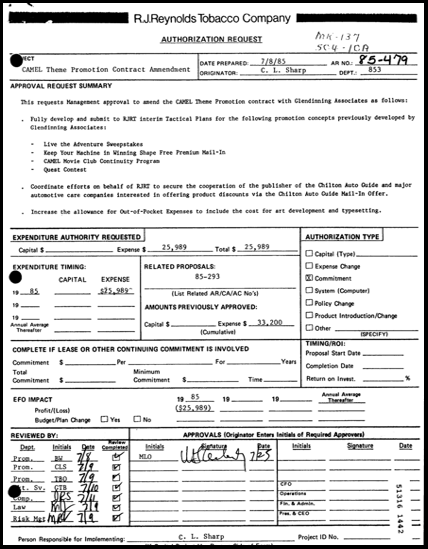
\includegraphics[width=\linewidth,height=4cm,keepaspectratio]{assets/Invoice.png}\\[0.12cm]
  \small Rechnung
\end{minipage}\hfill
\begin{minipage}[t]{0.23\textwidth}
  \centering
  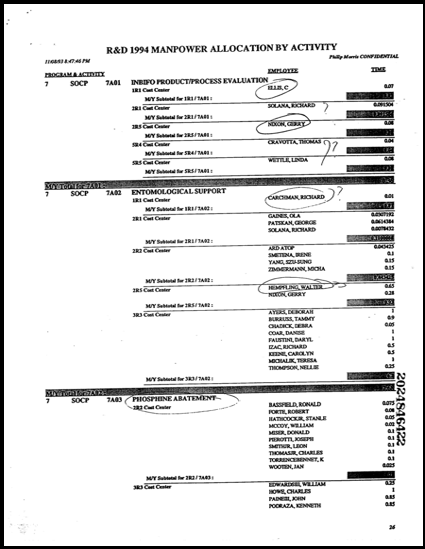
\includegraphics[width=\linewidth,height=4cm,keepaspectratio]{assets/budget.png}\\[0.12cm]
  \small Haushaltsplan
\end{minipage}\hfill
\begin{minipage}[t]{0.23\textwidth}
  \centering
  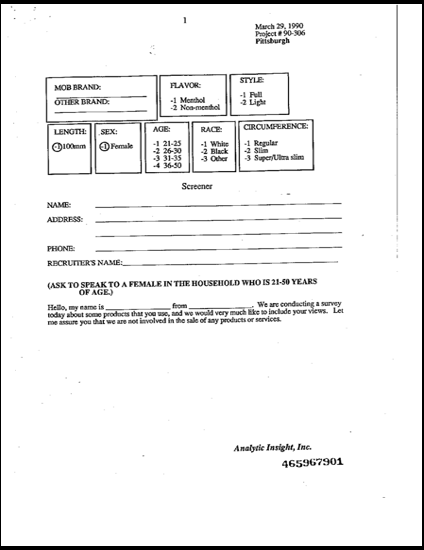
\includegraphics[width=\linewidth,height=4cm,keepaspectratio]{assets/Questionare.png}\\[0.12cm]
  \small Fragebogen
\end{minipage}\hfill
\begin{minipage}[t]{0.23\textwidth}
  \centering
  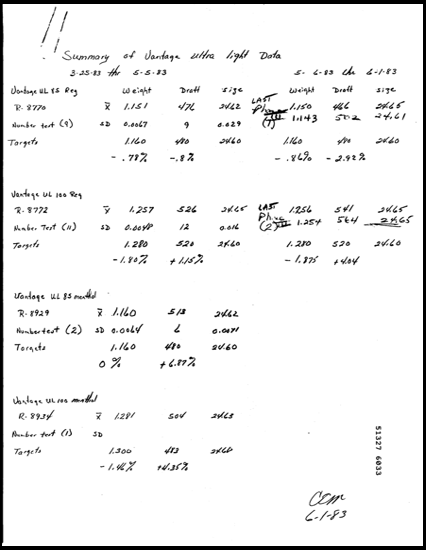
\includegraphics[width=\linewidth,height=4cm,keepaspectratio]{assets/Handwritten.png}\\[0.12cm]
  \small handschriftliches Formular
\end{minipage}

\vfill
\begin{flushright}
  \scriptsize\color{gray}Bildquelle: RVL-CDIP-Datensatz [2]
\end{flushright}
\end{frame}

% 3
\begin{frame}{Warum Textregionen automatisch erkannt werden sollen}
\begin{columns}[T]
\column{0.43\textwidth}
\textbf{Durchgängige Automatisierung}
\begin{itemize}
  \item Formulare werden als ganze Seiten erfasst.
  \item Vor OCR und Analyse müssen Textregionen lokalisiert werden.
  \item Manuelle Boxen bremsen die Automatisierung.
\end{itemize}

\vspace{0.5em}
\textbf{Ziel dieser Arbeit}
\begin{itemize}
  \item Textregionen automatisch erkennen
  \item zusätzliche manuelle Annotationen minimieren
\end{itemize}

\column{0.53\textwidth}
\begin{center}
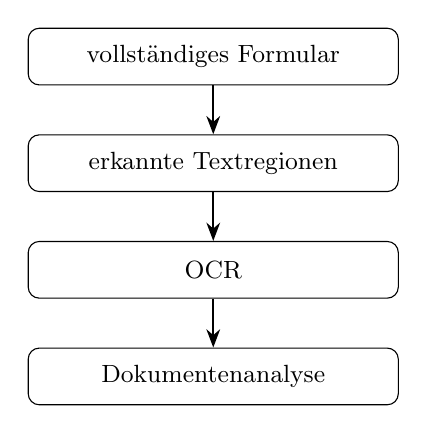
\begin{tikzpicture}[>=Stealth,node distance=0.62cm,font=\small]
  \node[draw,rounded corners,fill=white,minimum width=4.7cm,minimum height=0.72cm] (a) {vollständiges Formular};
  \node[draw,rounded corners,fill=white,below=of a,minimum width=4.7cm,minimum height=0.72cm] (b) {erkannte Textregionen};
  \node[draw,rounded corners,fill=white,below=of b,minimum width=4.7cm,minimum height=0.72cm] (c) {OCR};
  \node[draw,rounded corners,fill=white,below=of c,minimum width=4.7cm,minimum height=0.72cm] (d) {Dokumentenanalyse};
  \draw[->,thick] (a)--(b);
  \draw[->,thick] (b)--(c);
  \draw[->,thick] (c)--(d);
\end{tikzpicture}
\end{center}
\end{columns}
\takeaway{Je weniger manuelle Zwischenschritte nötig sind, desto besser lässt sich die gesamte Verarbeitung automatisieren.}
\end{frame}

% 4
\begin{frame}{Aufgabe: Textregionen statt Feldbedeutungen}
\begin{columns}[T]
\column{0.55\textwidth}
\begin{center}
\textbf{Beispielhafte Bounding Boxes um Textregionen}\\[0.25em]
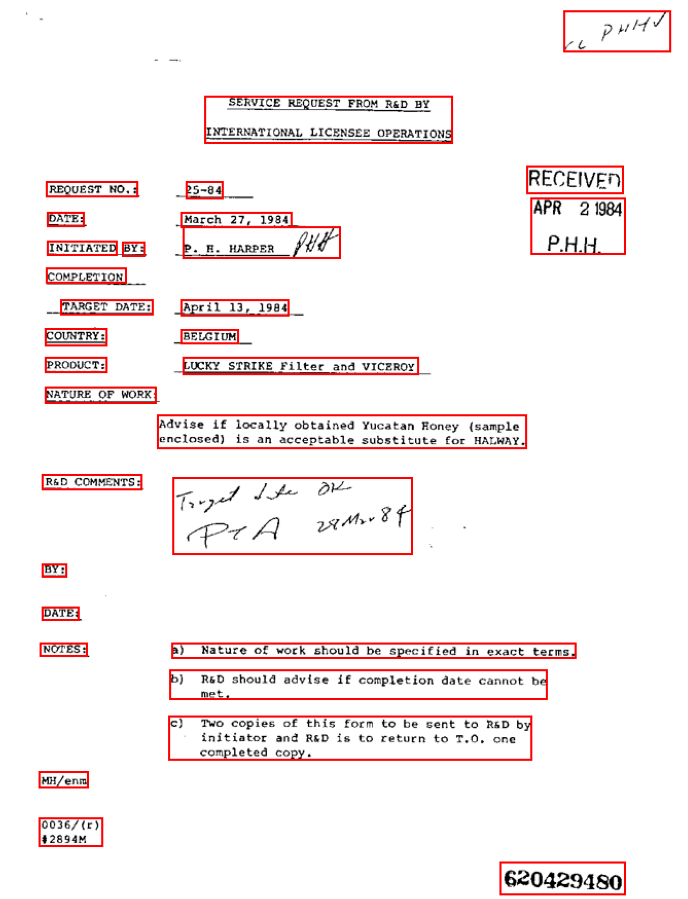
\includegraphics[height=4.9cm]{assets/Figure_2_qual.png}\\[0.1em]
\scriptsize\color{navy}Annotationsbeispiel aus FUNSD [1]
\end{center}

\column{0.40\textwidth}
\textbf{Erkennungsziel}
\begin{itemize}
  \item eine Klasse: \texttt{text}
  \item eine Bounding Box je zusammenhängendem Textabschnitt
  \item keine Klassen für Name, Datum oder Adresse
\end{itemize}

\takeaway{Erkannt wird die Position des Textes.}
\end{columns}
\end{frame}

% 5
\begin{frame}{Herausforderung: Annotationsaufwand und Realitätslücke}
\begin{columns}[T]
\column{0.48\textwidth}
\textbf{Manuelle Annotationen sind teuer}
\begin{itemize}
  \item Jede Textregion benötigt eine Bounding Box.
  \item Bounding Boxes müssen gezeichnet und geprüft werden.
  \item Neue Formulartypen erzeugen neuen Aufwand.
\end{itemize}

\column{0.48\textwidth}
\textbf{Synthetisch und real unterscheiden sich}
\begin{itemize}
  \item Synthetische Seiten liefern Boxen automatisch.
  \item Reale Seiten enthalten mehr Schriften, Handschrift, Logos und Scanrauschen.
  \item Ein rein synthetisch trainiertes Modell überträgt sich daher nicht vollständig.
\end{itemize}
\end{columns}

\vspace{0.7em}
\takeaway{Gesucht wird ein Verfahren, das reale Seiten nutzt, ohne für jede neue Seite manuelle Boxen zu verlangen.}
\end{frame}

% 6
\begin{frame}{Datengrundlage: FUNSD}
\begin{columns}[T]
\column{0.55\textwidth}
\begin{center}
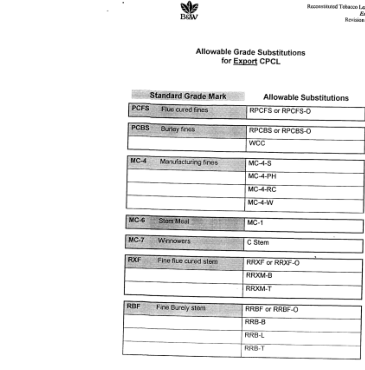
\includegraphics[height=5.1cm]{assets/real_form_tabular.png}
\end{center}

\column{0.40\textwidth}
\textbf{Form Understanding in Noisy Scanned Documents}
\begin{itemize}
  \item 199 vollständig annotierte Formulare
  \item 149 Trainings- und 50 Testformulare
  \item gerasterte Dokumente mit 100 dpi
  \item reales Druck- und Scanrauschen
\end{itemize}

\vspace{0.3em}
\textbf{Verwendung in dieser Arbeit}
\begin{itemize}
  \item synthetische Seiten aus Trainingslayouts
  \item Auswertung auf dem realen Testsatz
\end{itemize}
\end{columns}
\sourcefootnote{FUNSD-Datensatz [1].}
\end{frame}

% 7
\begin{frame}{Erzeugung synthetischer Trainingsseiten}
\begin{center}
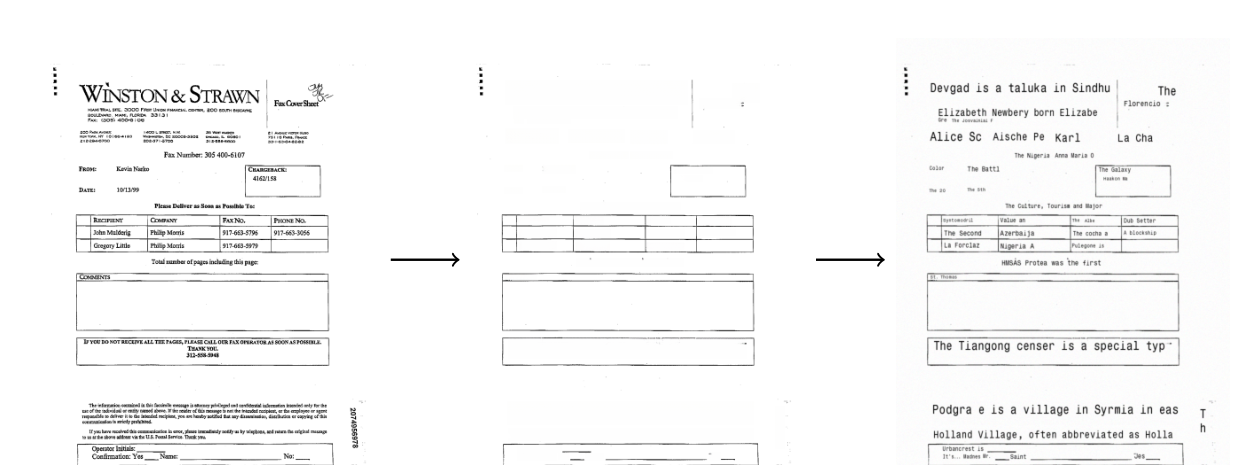
\includegraphics[width=0.94\linewidth]{assets/pipeline_crop.png}
\end{center}
\begin{enumerate}
  \item Vorhandene FUNSD-Boxen bestimmen die zu verändernden Textregionen.
  \item Inpaint Anything entfernt den ursprünglichen Text und rekonstruiert den Hintergrund.
  \item Wikipedia-Text wird passend umbrochen und in die Regionen eingesetzt.
  \item Die neuen Bounding Boxes werden automatisch gespeichert.
\end{enumerate}
\sourcefootnote{Inpaint Anything [5].}
\end{frame}

% 8
\begin{frame}{Detektor: Faster Region-Based Convolutional Neural Network}
\begin{columns}[T]
\column{0.43\textwidth}
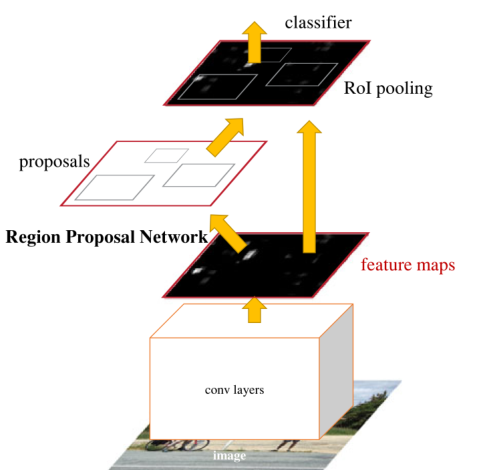
\includegraphics[width=0.98\linewidth]{assets/frcnn_crop.png}
\shortnote{Abbildung nach Ren et al. [3].}

\column{0.52\textwidth}
\begin{enumerate}
  \item \textbf{Feature Extraction}\\
  ResNet-50 berechnet lokale Features; das FPN stellt mehrere Skalen bereit.

  \item \textbf{Region Proposals}\\
  Das RPN erzeugt Kandidatenbereiche, die wahrscheinlich Text enthalten.

  \item \textbf{RoI Align}\\
  Features unterschiedlich großer Proposals werden vereinheitlicht.

  \item \textbf{Classification und Box Regression}\\
  Text oder Hintergrund; Position und Größe der Bounding Box werden angepasst.

  \item \textbf{Final Detections}\\
  NMS entfernt stark überlappende doppelte Predictions.
\end{enumerate}
\end{columns}
\end{frame}

% 9
\begin{frame}{Wie entstehen Region Proposals?}
\begin{columns}[T]
\column{0.47\textwidth}
\begin{center}
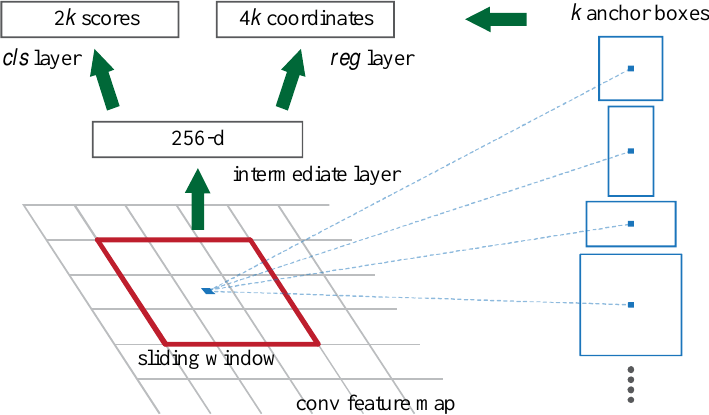
\includegraphics[width=\linewidth]{assets/rpn_ren_fig3_left.png}
\end{center}
\shortnote{Ren et al. [3], Fig. 3 (Ausschnitt; Paper-Konfiguration).}

\column{0.49\textwidth}
\textbf{Die Grafik wird von unten nach oben gelesen.}
\vspace{0.25em}
\begin{enumerate}\small
  \item \textbf{Feature Map und Sliding Window}\\
  Das kleine Netz wird an jede räumliche Position gesetzt.
  \item \textbf{$k$ Anchor Boxes}\\
  Ausgangsboxen decken verschiedene Größen und Seitenverhältnisse ab.
  \item \textbf{Objectness}\\
  Für jeden Anchor wird Objekt oder Hintergrund geschätzt.
  \item \textbf{Box Regression}\\
  Vier Werte verschieben und skalieren den Anchor zu einem Proposal.
  \item \textbf{Auswahl}\\
  Hohe Scores bleiben; NMS entfernt stark überlappende Proposals.
\end{enumerate}
\end{columns}
\takeaway{Das RPN erzeugt Kandidatenboxen; die endgültige Klassenentscheidung folgt im Detection Head.}
\end{frame}

% 10
\begin{frame}{Auswertung der Erkennungen}
\begin{center}
\EvaluationTable
\end{center}

\vspace{0.35em}
\begin{center}
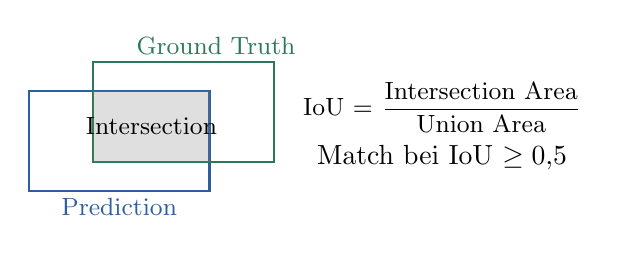
\begin{tikzpicture}[scale=0.82]
  \draw[thick,blueaccent] (0,0) rectangle (2.8,1.55);
  \draw[thick,greenaccent] (1.0,0.45) rectangle (3.8,2.0);
  \fill[gray,opacity=0.25] (1.0,0.45) rectangle (2.8,1.55);
  \node[blueaccent] at (1.4,-0.25) {\small Prediction};
  \node[greenaccent] at (2.9,2.25) {\small Ground Truth};
  \node at (1.9,1.0) {\small Intersection};
  \node[align=center] at (6.4,1.0) {\small
    IoU $=$ $\dfrac{\text{Intersection Area}}{\text{Union Area}}$\\[0.35em]
    Match bei IoU $\geq 0{,}5$};
\end{tikzpicture}
\end{center}
\sourcefootnote{IoU-Grenzwert entsprechend der FUNSD-Auswertung [1].}
\end{frame}

% 11
\begin{frame}{Self-Training: Teacher und Student}
\begin{center}
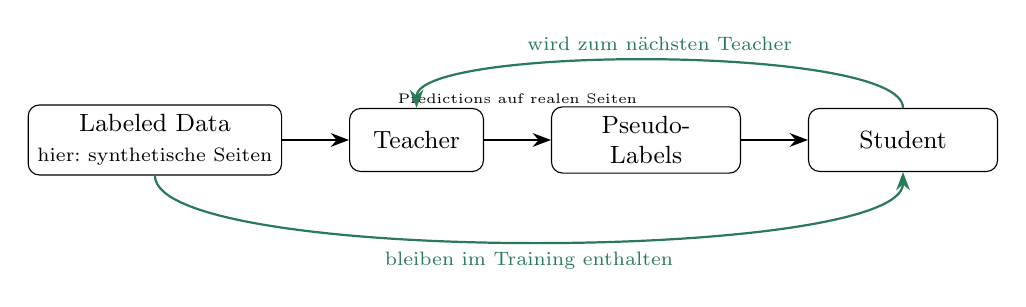
\begin{tikzpicture}[>=Stealth,node distance=0.85cm,font=\small]
  \node[draw,rounded corners,fill=white,align=center,minimum width=2.8cm,minimum height=0.8cm] (a) {Labeled Data\\{\scriptsize hier: synthetische Seiten}};
  \node[draw,rounded corners,fill=white,right=of a,minimum width=1.7cm,minimum height=0.8cm] (b) {Teacher};
  \node[draw,rounded corners,fill=white,right=of b,align=center,minimum width=2.4cm,minimum height=0.8cm] (c) {Pseudo-\\Labels};
  \node[draw,rounded corners,fill=white,right=of c,align=center,minimum width=2.4cm,minimum height=0.8cm] (d) {Student};
  \draw[->,thick] (a)--(b);
  \draw[->,thick] (b)--node[above=0.33cm,font=\tiny,align=center]{Predictions auf realen Seiten}(c);
  \draw[->,thick] (c)--(d);
  \draw[->,thick,greenaccent] (a.south) .. controls +(0,-1.15) and +(0,-1.15) .. node[below,font=\scriptsize]{bleiben im Training enthalten} (d.south);
  \draw[->,thick,greenaccent] (d.north) .. controls +(0,0.8) and +(0,0.8) .. node[above,font=\scriptsize]{wird zum nächsten Teacher} (b.north);
\end{tikzpicture}
\end{center}

\vspace{0.55em}
\begin{itemize}
  \item Der Teacher erzeugt Pseudo-Labels für reale, nicht annotierte Seiten.
  \item Der Student lernt aus synthetischen Seiten mit Ground Truth und realen Seiten mit Pseudo-Labels.
  \item Die ursprünglichen synthetischen Daten bleiben in jeder regulären Runde erhalten.
\end{itemize}
\takeaway{Reale Daten werden nutzbar, ohne für jede Seite neue manuelle Bounding Boxes zu zeichnen.}
\end{frame}

\begin{frame}{ASTOD: Originalmethode}
\begin{center}
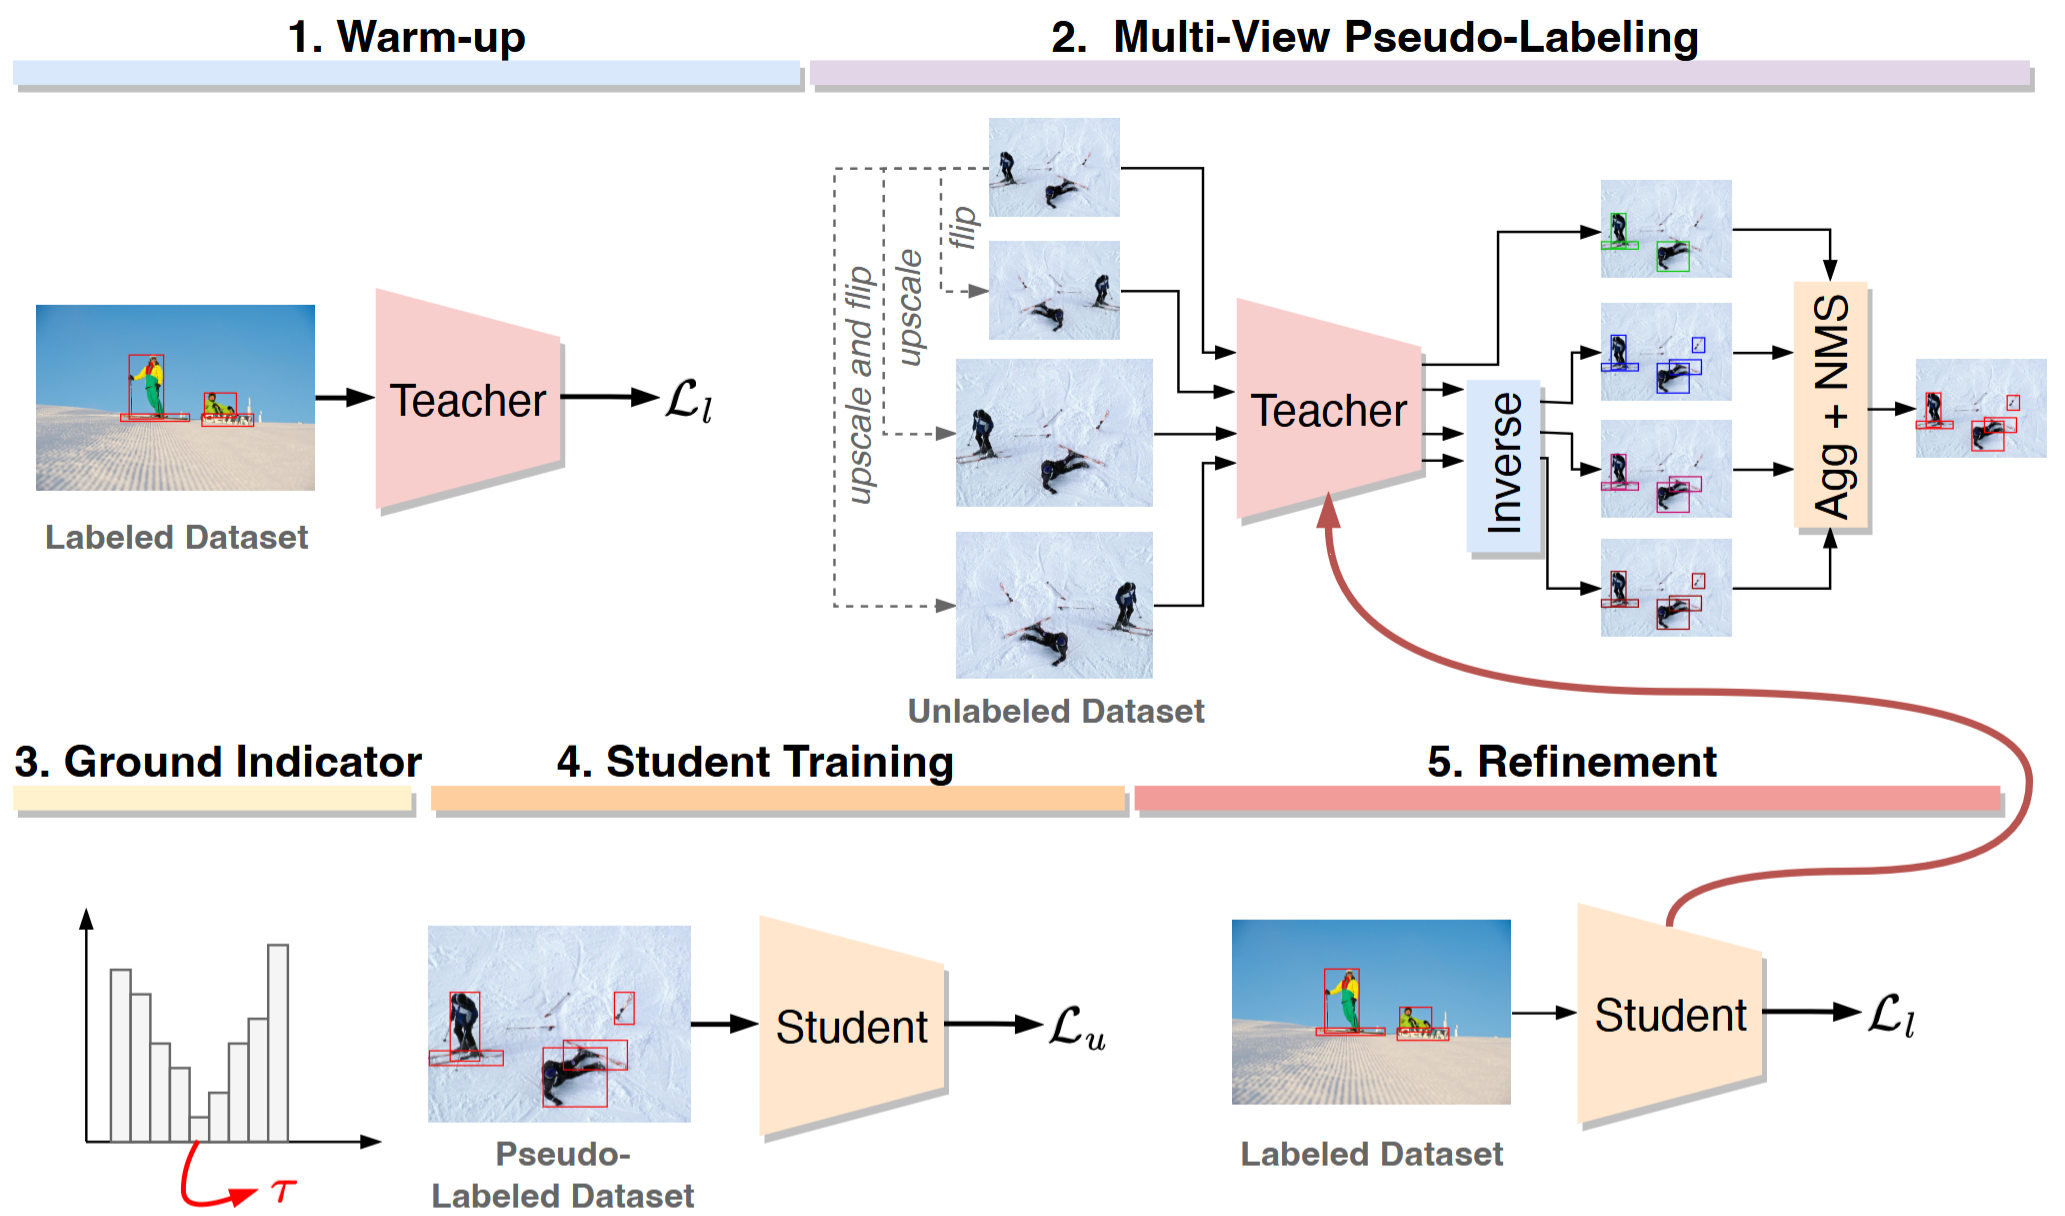
\includegraphics[width=0.68\linewidth]{assets/astod_loop_full_steps.png}
\end{center}

\vspace{-0.35em}

\begin{itemize}\scriptsize
  \item Zuerst wird ein Teacher auf gelabelten Daten trainiert.
  \item Der Teacher erzeugt Predictions für mehrere Ansichten der ungelabelten Bilder, beispielsweise gespiegelt oder vergrößert.
  \item Die Predictions werden zurücktransformiert und mit NMS zu gemeinsamen Boxen zusammengeführt.
  \item Ein adaptiver Confidence Threshold aus dem Score-Histogramm filtert unsichere Pseudo-Labels.
  \item Der Student lernt aus gelabelten und gewichteten pseudo-gelabelten Daten; nach Refinement wird Student zu Teacher.
\end{itemize}

\sourcefootnote{ASTOD-Pipeline nach Vandeghen et al. [4].}
\end{frame}

% 13
\begin{frame}{Übertragung von ASTOD auf diese Arbeit}
\begin{columns}[T]
\column{0.55\textwidth}
\begin{center}
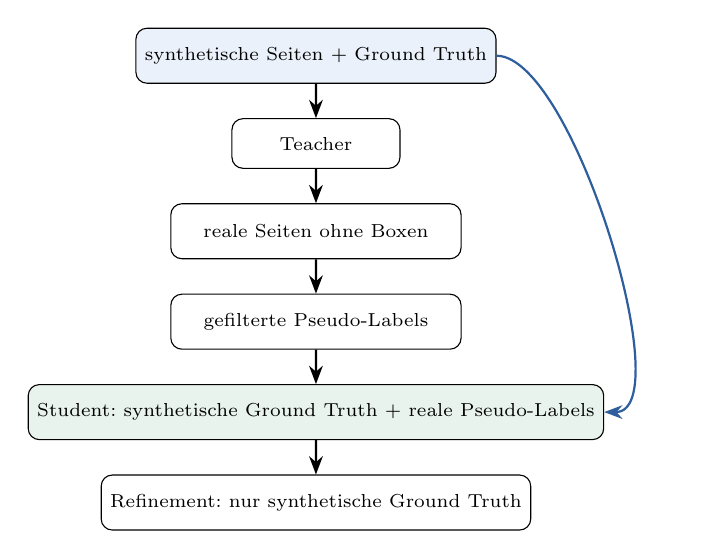
\begin{tikzpicture}[>=Stealth,node distance=0.45cm,font=\scriptsize,scale=0.97,transform shape]
  \node[draw,rounded corners,fill=softblue,align=center,minimum width=3.8cm,minimum height=0.72cm] (s) {synthetische Seiten + Ground Truth};
  \node[draw,rounded corners,fill=white,below=of s,minimum width=2.2cm,minimum height=0.65cm] (t) {Teacher};
  \node[draw,rounded corners,fill=white,below=of t,align=center,minimum width=3.8cm,minimum height=0.72cm] (r) {reale Seiten ohne Boxen};
  \node[draw,rounded corners,fill=white,below=of r,align=center,minimum width=3.8cm,minimum height=0.72cm] (p) {gefilterte Pseudo-Labels};
  \node[draw,rounded corners,fill=softgreen,below=of p,align=center,minimum width=4.6cm,minimum height=0.72cm] (u) {Student: synthetische Ground Truth + reale Pseudo-Labels};
  \node[draw,rounded corners,fill=white,below=of u,align=center,minimum width=4.6cm,minimum height=0.72cm] (f) {Refinement: nur synthetische Ground Truth};
  \draw[->,thick] (s)--(t);
  \draw[->,thick] (t)--(r);
  \draw[->,thick] (r)--(p);
  \draw[->,thick] (p)--(u);
  \draw[->,thick,blueaccent] (s.east) .. controls +(1.0,0) and +(1.0,0) .. (u.east);
  \draw[->,thick] (u)--(f);
\end{tikzpicture}
\end{center}

\column{0.40\textwidth}
\textbf{Zuordnung in dieser Arbeit}
\begin{itemize}
  \item Labeled Data $\rightarrow$ synthetische Seiten mit Ground Truth
  \item Unlabeled Data $\rightarrow$ reale FUNSD-Trainingsseiten
  \item Student $\rightarrow$ beide Datengruppen
  \item Refinement $\rightarrow$ erneut nur synthetische Daten
\end{itemize}

\vspace{0.3em}
\textbf{Wichtige Abweichung}
\begin{itemize}
  \item ASTOD nimmt dieselbe Datenverteilung an.
  \item Hier wird eine Lücke zwischen synthetischen und realen Daten überbrückt.
\end{itemize}
\end{columns}
\end{frame}

% 14
\begin{frame}{Versuchsaufbau}
\begin{center}
\SetupTable
\end{center}
\takeaway{Detektor und Auswertung bleiben in den Hauptvergleichen gleich; verändert wird die Trainingsstrategie.}
\end{frame}

% 15
\begin{frame}{Hyperparameter Search}
\experimentquestion{Welche stabile Optimizer-Einstellung wird für die folgenden Vergleiche verwendet?}
\begin{columns}[T]
\column{0.49\textwidth}
\textbf{Ausgangspunkt und Anpassung}
\begin{itemize}
  \item Ausgangswerte orientieren sich an FUNSD und Faster R-CNN.
  \item In dieser Arbeit werden mehrere Werte systematisch verglichen.
  \item Danach bleibt eine Einstellung für die Hauptversuche fest.
\end{itemize}

\vspace{0.3em}
\small
FUNSD liefert den Ausgangspunkt; die endgültigen Werte stammen aus der eigenen Hyperparameter Search.

\column{0.47\textwidth}
\textbf{Gewählte Einstellung}
\begin{center}
\begin{tabular}{lc}
\toprule
Parameter & Wert \\
\midrule
Learning Rate & 0{,}006 \\
Momentum & 0{,}8 \\
Weight Decay & 0{,}0005 \\
\bottomrule
\end{tabular}
\end{center}

\vspace{0.45em}
\begin{itemize}
  \item Learning Rate: Stärke der Gewichtsänderung
  \item Momentum: glättet die Update-Richtung
  \item Weight Decay: begrenzt zu große Gewichte
\end{itemize}
\end{columns}
\sourcefootnote{Ausgangswerte nach FUNSD [1] und Faster R-CNN [3]; Auswahl durch eigene Versuche.}
\end{frame}

% 16
\begin{frame}{Ausgangsleistung ohne Self-Training}
\experimentquestion{Wie groß ist die Lücke vor dem Self-Training?}
\begin{center}
\BaselineTable
\end{center}
\vspace{0.45em}
\begin{center}
\textbf{Auswertung:} reale FUNSD-Testformulare
\end{center}
\takeaway{Das synthetisch trainierte Modell liegt 0{,}10 F1 unter dem Modell mit realen Annotationen.}
\end{frame}

% 17
\begin{frame}{Entwicklung über viele Self-Training-Runden}
\experimentquestion{Wie verändert sich die Leistung über weitere Teacher-Student-Runden?}
\begin{center}
\begin{tikzpicture}
  \node[inner sep=0] (img) {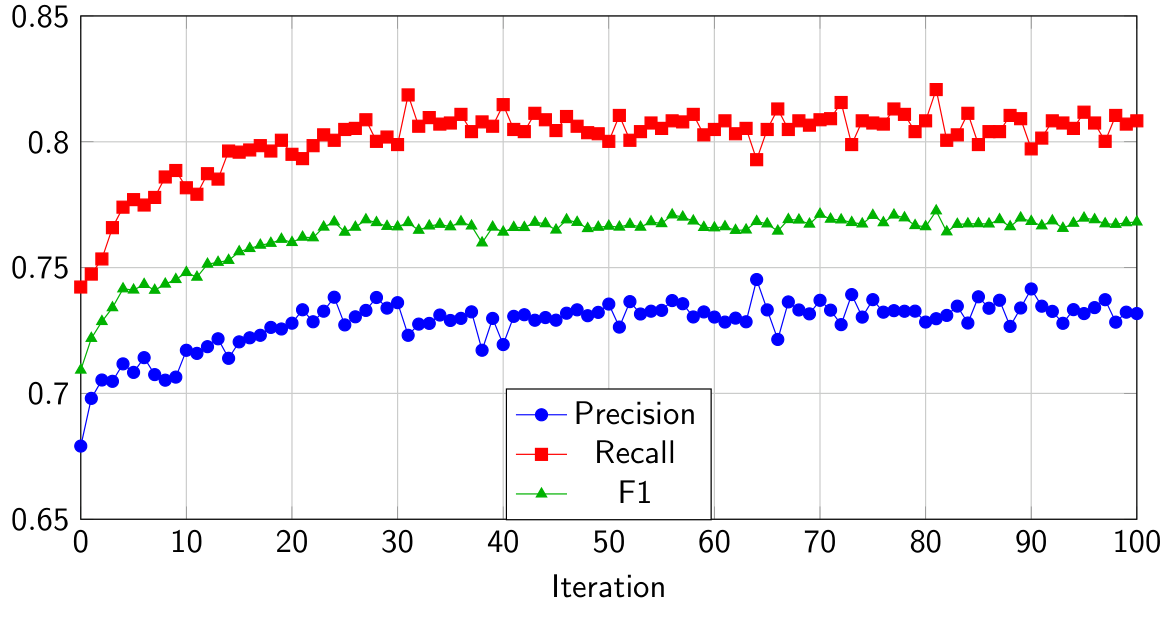
\includegraphics[width=0.88\linewidth]{assets/selftraining100_fullchart.png}};
  \node[draw=greenaccent,rounded corners,fill=white,text=navy,font=\bfseries\scriptsize] at ($(img.south east)+(-1.9cm,2.45cm)$) {Maximum: F1 $=0{,}7726$};
\end{tikzpicture}
\end{center}
\vspace{-0.1em}
\begin{center}\small
F1 steigt von etwa 0{,}708 auf 0{,}773. Der größte Zuwachs entsteht früh, danach folgt ein Plateau.
\end{center}
\end{frame}

% 18
\begin{frame}{Zwei Varianten der synthetischen Seiten}
\begin{columns}[T]
\column{0.49\textwidth}
\begin{center}
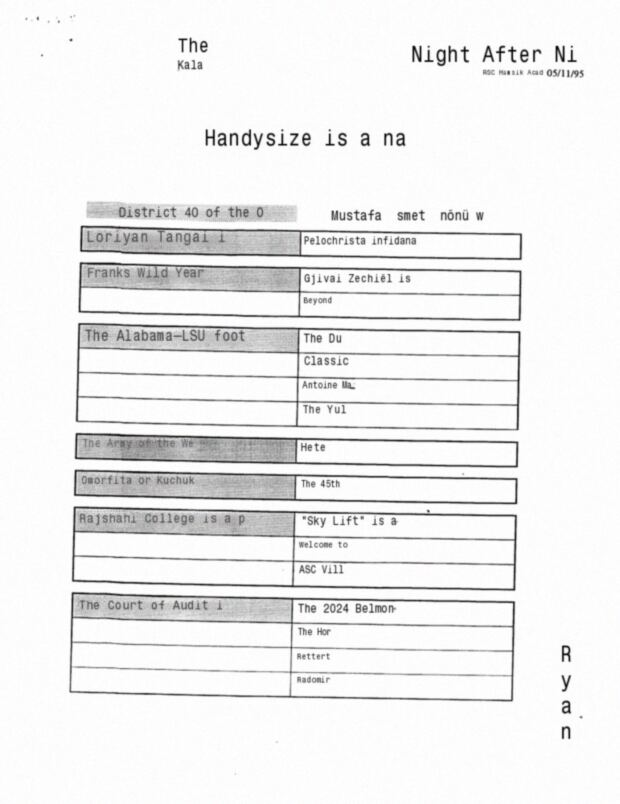
\includegraphics[height=5.75cm]{assets/inpainted_example_compact.jpg}\\[0.15em]
\textbf{Rekonstruierter Hintergrund}
\end{center}
\centering
{\scriptsize Der alte Text wird entfernt; neuer Text wird direkt in den rekonstruierten Bereich eingesetzt.}

\column{0.49\textwidth}
\begin{center}
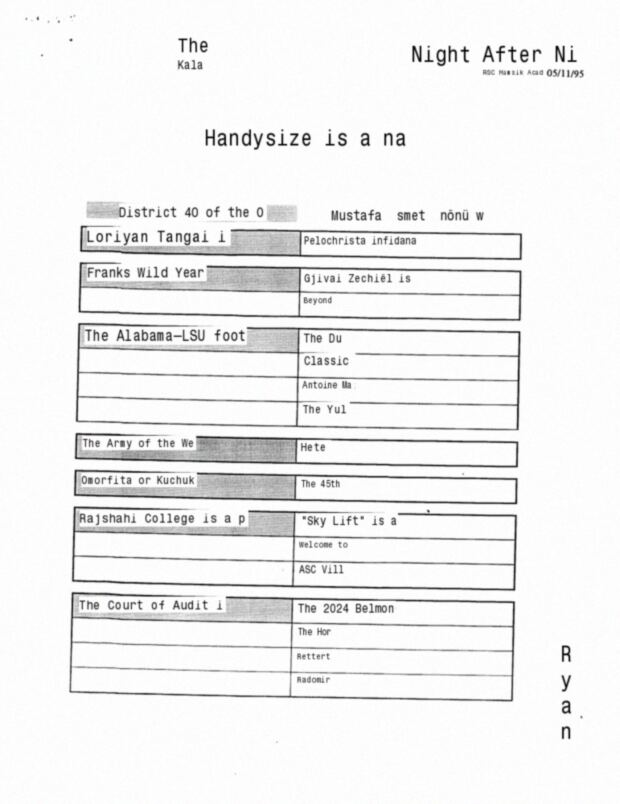
\includegraphics[height=5.75cm]{assets/white_example_compact.jpg}\\[0.15em]
\textbf{Weißer Hintergrund}
\end{center}
\centering
{\scriptsize Die ursprüngliche Textregion wird vor dem Einsetzen des neuen Textes durch ein weißes Rechteck ersetzt.}
\end{columns}
\end{frame}

% 19
\begin{frame}{Vergleich der Erzeugungsverfahren}
\experimentquestion{Hilft der erhaltene Scan-Hintergrund bei der Übertragung auf reale Formulare?}
\begin{center}
\GenerationTable
\end{center}
\vspace{0.55em}
\takeaway{Direktes Einfügen in den rekonstruierten Hintergrund ist leicht besser; der Unterschied bleibt klein.}
\end{frame}

% 20
\begin{frame}{Einfluss der Menge synthetischer Daten}
\experimentquestion{Wie viele synthetische Seiten werden für nützliches Self-Training benötigt?}
\begin{center}
\SyntheticAmountTable
\end{center}
\vspace{0.45em}
\takeaway{Auch kleinere Teilmengen sind nutzbar.}
\end{frame}

% 21
\begin{frame}{Ablation: synthetische Daten entfernen}
\experimentquestion{Kann die synthetische Grundlage nach Erreichen des Plateaus entfallen?}
\small
Fünf starke Checkpoints aus dem Plateau werden auf zwei Arten verglichen:
\begin{center}
\AnchorTable
\end{center}
\vspace{0.25em}
\begin{itemize}
  \item \textbf{Regular:} Student lernt aus synthetischen Seiten und realen Pseudo-Labels; danach folgt synthetisches Refinement.
  \item \textbf{Pseudo-only:} Ab dem gewählten Checkpoint bleiben nur reale Pseudo-Labels; das Refinement entfällt.
\end{itemize}
\takeaway{Das Entfernen der synthetischen Daten senkt F1 in allen getesteten Fortsetzungen.}
\end{frame}

% 22
\begin{frame}{Synthetische Daten bei realer Aufsicht}
\experimentquestion{Helfen synthetische Daten noch, wenn reale Annotationen vorhanden sind?}
\begin{center}
\RealSupervisionTable
\end{center}
\vspace{0.55em}
\takeaway{Direktes Mischen liefert keinen Gewinn; die Einbindung über Self-Training verbessert F1 hierf.}
\end{frame}

% 23
\begin{frame}{Zentrale Ergebnisse}
\begin{enumerate}
  \item Nur synthetische Daten erreichen \textbf{0{,}70 F1}; reale Annotationen \textbf{0{,}80 F1}.
  \item Synthetisch-reales Self-Training erhöht F1 auf \textbf{0{,}77}.
  \item Das Entfernen der synthetischen Grundlage verschlechtert die getesteten Fortsetzungen.
  \item Mit realen Annotationen erreicht synthetisch unterstütztes Self-Training \textbf{0{,}814 F1}.
\end{enumerate}
\takeaway{Self-Training verkleinert die Lücke zwischen synthetischen und realen Daten, ersetzt reale Annotationen aber nicht.}
\end{frame}

% 24
\begin{frame}{Grenzen der Untersuchung}
\begin{itemize}
  \item Auswertung auf einem Formulardatensatz und einer Erkennungsklasse
  \item Wiederverwendung annotierter Ausgangslayouts für synthetische Seiten
  \item begrenzte Variation bei Schriftarten und Handschrift
  \item keine Mittelung über mehrere unabhängige Zufallsinitialisierungen
  \item kein eigener Validierungssatz für die Modellauswahl
\end{itemize}
\end{frame}

% 25
\begin{frame}{Fazit und Ausblick}
\textbf{Fazit}
\begin{itemize}
  \item Synthetische Daten bilden einen brauchbaren automatischen Ausgangspunkt.
  \item Self-Training nutzt reale Seiten ohne zusätzliche manuelle Boxen.
  \item Die synthetische Ground Truth stabilisiert die wiederholten Trainingsrunden.
  \item Reale Annotationen liefern weiterhin die stärkste Aufsicht.
\end{itemize}

\vspace{0.45em}
\textbf{Ausblick}
\begin{itemize}
  \item realistischere Schriften, Handschrift und Layoutvariation
  \item weitere Datensätze und neuere Detektoren
  \item mehrere Zufallsinitialisierungen und eigener Validierungssatz
\end{itemize}
\end{frame}

% 26
\begin{frame}{Literatur}
\footnotesize
\begin{enumerate}
  \item G. Jaume, H. K. Ekenel und J.-P. Thiran, ``FUNSD: A Dataset for Form Understanding in Noisy Scanned Documents'', ICDAR Workshops, 2019.
  \item A. W. Harley, A. Ufkes und K. G. Derpanis, ``Evaluation of Deep Convolutional Nets for Document Image Classification and Retrieval'', ICDAR, 2015.
  \item S. Ren, K. He, R. Girshick und J. Sun, ``Faster R-CNN: Towards Real-Time Object Detection with Region Proposal Networks'', IEEE TPAMI, 2017.
  \item R. Vandeghen et al., ``Adaptive Self-Training for Object Detection'', ICCV Workshops, 2023.
  \item T. Yu et al., ``Inpaint Anything: Segment Anything Meets Image Inpainting'', arXiv:2304.06790, 2023.
\end{enumerate}
\end{frame}

\end{document}
